\section{Reaching a flat endpoint with an infinite chain of cells}
\label{sec:radial-tails}
\label{sec:radial-selection}

By Proposition~\ref{prop:obs-monotone-tail} the profile must have
infinitely many turning circles near each endpoint. We obtain them by
repeating one Morse cell infinitely often, with rapidly shrinking
lengths and heights. This section constructs such a \emph{tail} and
analyses the equation $L_ju=0$ on it. Its results are the following.
\begin{itemize}
\item The tail is a smooth profile which extends by zero across the
 endpoint, with explicit bounds on all coefficients
 (Lemmas~\ref{lem:cell} and~\ref{lem:tail-flat}).
\item On the part of the tail which is deep enough for a given
 frequency $j$, the equation reduces \emph{exactly} to a three-term
 recurrence with a dominant diagonal. Hence there is a unique solution
 decaying towards the endpoint, it loses the factor
 $e^{-2n^2+o(n^2)}$ across cell $n$, and the operator has a bounded
 inverse (Lemma~\ref{lem:radial-deep-inverse}).
\item The accumulated loss $e^{-2n^3/3}$ beats every fixed number of
 derivatives, so the decaying solution is flat at the endpoint.
\item The heights of the cells can be chosen so that, at every
 frequency, the decaying solution is quantitatively transverse to the
 solution arriving from the interior
 (Lemma~\ref{lem:radial-product-selection}).
\end{itemize}

\subsection{The budget of lengths, heights and errors}

For $n\ge N$ let $d_n$ be the least integer which is not a square and
is at least $e^{n^2}$; thus $d_n=e^{n^2}+O(1)$. Let $A_n$ and $B_n$ be
the Morse parameters \eqref{eq:rad-eq-rm5} for $d=d_n$, so that
\[
 A_n\asymp e^{-n^2},\qquad B_n=d_n^{-9}\asymp A_n^9 .
\]
The height of cell $n$ is
\begin{equation}\label{eq:rad-eq-js2}
 \lambda_n=e^{-n^{5/2}}\prod_{k=N}^n\sigma_k,
 \qquad 1\le\sigma_k\le2 .
\end{equation}
The \emph{height ratios} $\sigma_k$ are free parameters until
Section~\ref{subsec:height-selection}; they change $\log\lambda_n$ by
at most $O(n)$, which does not affect any of the comparisons of scales
below. The initial index $N$ will be taken large.

Table~\ref{tab:endpoint-budget} lists the scales and the reason for
each. The choices can be understood before any computation. A
derivative of fixed order on a cell of length $e^{-n^2}$ costs
$e^{C_sn^2}$. For the profile to be flat its amplitude must decay
faster than that, and the exponent $n^{5/2}$ achieves it. The solution
must decay faster still, in order to pay for reciprocals of the
coefficients; its cubic exponent is not chosen but comes out of the
recurrence. These requirements leave the whole interval $2<5/2<3$ for
the middle exponent; no optimal value is singled out.

\begin{table}[htbp]
\centering
\begin{tabularx}{\linewidth}{@{}l l Y@{}}
\toprule
Quantity & Size & Purpose\\
\midrule
Length of cell $n$ & $A_n\asymp e^{-n^2}$ &
 The lengths are summable, so the cells accumulate at a finite
 endpoint.\\
Height of cell $n$ & $\lambda_n=e^{-n^{5/2}+O(n)}$ &
 Beats the cost $e^{C_sn^2}$ of $s$ derivatives: the profile is
 flat.\\
Length of a join & $\asymp A_n^{12}$ &
 A large change of height is crossed with negligible transfer
 error.\\
Matching angle & $\delta_n=c_0e^{-n^2}$ &
 The excluded sets of height ratios are summable over all frequency
 bands.\\
Decay of the solution & $H_n=e^{-S_n}$, $S_n=\tfrac23n^3$ &
 Produced by the recurrence; gives integrability and flatness of the
 selected solution.\\
Coefficient allowance & $\mathcal E_n=e^{n^{5/2}\log(e+n)}$ &
 Absorbs fixed powers of coefficients and of changes of coordinates,
 while staying below $e^{\varepsilon S_n}$.\\
\bottomrule
\end{tabularx}
\caption{The scales of the tail. Their compatibility is expressed by
\eqref{eq:rad-scale-separation} and verified in this section.}
\label{tab:endpoint-budget}
\end{table}

All comparisons of scales concern a fixed number of derivatives. No
bound is claimed to be uniform as the order of differentiation tends
to infinity.

\subsection{One cell}
\label{subsec:one-cell}

Let $A=A_n$, $B=B_n$ and $\rho=A(e^{-X}-e^{-2X})-B$. Let $X_L<X_R$ be
the two zeros of $\rho$; then $X_L=O(B/A)$ and
$X_R=\log(A/B)+O(B/A)$. With $\mathcal P=1$, Lemma~\ref{lem:liouville}
says that a positive increasing solution $r$ of
\begin{equation}\label{eq:rad-eq-rm4}
 r_{XX}=-\rho\,r,\qquad\text{together with}\qquad w=\lambda\,r_X,
\end{equation}
defines a profile on which $L_j=-(\lambda/r_X)\,H_{j,M}$. We take the
solution with
\[
 r(X_R)=1,\qquad r_X(X_R)=\epsilon_RA^5,
\]
for a fixed small $\epsilon_R>0$, and we retain the interval
\[
 X_c\le X\le X_R+c_RA^{-4},\qquad X_c=-\log\tfrac32,
\]
for a fixed sufficiently small $c_R>0$. It consists of three parts
(Figure~\ref{fig:cell}):
\begin{itemize}
\item the \emph{short positive cap} $[X_c,X_L]$, where $\rho<0$ and
 $w$ rises;
\item the \emph{negative component} $(X_L,X_R)$, where $\rho>0$ and
 $w$ falls; its length in $X$ is about $\log(A/B)\asymp n^2$;
\item the \emph{long positive cap} $[X_R,X_R+c_RA^{-4}]$, where
 $-B\le\rho<0$ and $w$ rises slowly.
\end{itemize}

\begin{figure}[htbp]
\centering
\begin{tikzpicture}[x=1cm,y=1cm,>=Stealth,font=\small]
\fill[teal!9] (.5,0) rectangle (2.3,2.9);
\fill[orange!12] (2.3,0) rectangle (6.4,2.9);
\fill[teal!9] (6.4,0) rectangle (10.4,2.9);
\fill[teal!22] (10.4,0) rectangle (11.3,2.9);
\draw[->] (0,0)--(12.4,0) node[right] {$r$};
\draw[thick,blue!70!black]
 (.5,1.55) .. controls (1.2,1.8) and (1.8,2.15) .. (2.3,2.2)
 .. controls (3.4,2.3) and (4.9,.5) .. (6.4,.42)
 .. controls (7.8,.36) and (9.4,.62) .. (10.4,.72)
 .. controls (10.75,.76) and (11.0,2.0) .. (11.3,2.5);
\draw[thick,blue!70!black,dashed] (11.3,2.5)--(11.9,2.75);
\draw[thick,blue!70!black,dashed] (.05,1.4)--(.5,1.55);
\foreach \x/\lab in {.5/X_c,2.3/X_L,6.4/X_R}{
 \draw (\x,-.08)--(\x,.08); \node[below] at (\x,-.08) {$\lab$};}
\draw (10.4,-.08)--(10.4,.08);
\node[below] at (10.2,-.08) {$X_R+c_RA^{-4}$};
\node[align=center] at (1.4,3.35) {short\\positive cap};
\node[align=center] at (4.35,3.35) {negative\\component};
\node[align=center] at (8.4,3.35) {long\\positive cap};
\node[align=center] at (10.85,3.35) {join};
\node at (1.4,.9) {$\rho<0$};
\node at (4.0,.9) {$\rho>0$};
\node at (8.4,1.4) {$-B\le\rho<0$};
\node[blue!70!black] at (3.3,2.55) {$w$};
\draw[decorate,decoration={brace,mirror,amplitude=5pt}]
 (.5,-.75)--(6.4,-.75) node[midway,below=6pt] {$I_n$: mass interval};
\draw[decorate,decoration={brace,mirror,amplitude=5pt}]
 (6.4,-.75)--(11.3,-.75) node[midway,below=6pt] {$J_n$: resistance interval};
\end{tikzpicture}
\caption{One cell and the join following it, in the direction of
increasing $r$ (not to scale). The tick marks give the values of the
model coordinate $X$. Each of the three parts of the cell has radial
length comparable to $A_n$; the join has length comparable to
$A_n^{12}$ or $A_{n\pm1}^{12}$. Along the join the profile rises by a
factor $e^{4n^2+o(n^2)}$. The intervals $I_n$ and $J_n$ are used in
Section~\ref{subsec:mass-resistance}.}
\label{fig:cell}
\end{figure}

\begin{lemma}[The cell is a radial profile]\label{lem:cell}
On the retained interval $r_X>0$. More precisely, with constants
independent of $n$,
\begin{equation}\label{eq:rad-eq-rm6a}
 r_X(X_c)=\tfrac38A+O(A^2),\qquad
 r(X_c)=1-\tfrac{15}{16}A+O(A^2),
\end{equation}
and
\begin{equation}\label{eq:rad-eq-rm6}
 \begin{gathered}
 r=1+O(A),\qquad cA^5\le r_X\le CA,\qquad
 r_X\asymp A^5\ \text{on the long positive cap},\\
 \Delta r\asymp A,\qquad
 \int_{X_c}^{X_R}r_X^2\,dX\asymp A^2,\qquad
 \int_{\text{each positive cap}}\sqrt{-\rho}\,dX\asymp\sqrt A .
 \end{gathered}
\end{equation}
Here $\Delta r$ is the radial length of each of the three parts.
\end{lemma}

\begin{proof}
On $[X_c,X_R]$ the integral $\int(Y-X_c)|\rho(Y)|\,dY$ is $O(A)$, so
the Volterra equation
\[
 r(X)=1-r_X(X_R)\,(X_R-X)
       -\int_X^{X_R}(Y-X)\,\rho(Y)\,r(Y)\,dY
\]
gives $r=1+O(A)$ there. For \eqref{eq:rad-eq-rm6a} evaluate the leading
terms with $t=e^{-Y}$:
\[
 \int_0^{3/2}(1-t)\,dt=\frac38,\qquad
 \int_0^{3/2}\log\frac{3/2}{t}\,(1-t)\,dt=\frac{15}{16};
\]
the constant $B$ contributes only $O(B\log^2(A/B))=o(A^2)$.

On the negative component $r_X(X)=r_X(X_R)+\int_X^{X_R}\rho\,r>0$. On
the short positive cap $r_{XX}=-\rho r>0$, so the minimum of $r_X$ is
its value at $X_c$, which is positive by \eqref{eq:rad-eq-rm6a}. On
the long positive cap $0<r_{XX}\le Br$; since
$B\cdot c_RA^{-4}\asymp c_RA^5$, comparison with $r_{XX}=Br$ shows
$r_X\asymp A^5$ there, and $r$ changes by $O(A)$. Taking $c_R$ small
keeps $r$ in a fixed positive range throughout. The remaining
statements follow by integration: $r_X\asymp A$ on a fixed part of
$[X_c,X_R]$ and $r_X\le CAe^{-X}+CA^5$ on all of it; on the long cap
$-\rho\asymp B$ away from $X_R$ and $\sqrt B\,A^{-4}\asymp\sqrt A$; on
the short cap $-\rho\asymp A$ on a fixed subinterval.
\end{proof}

The last quantity in \eqref{eq:rad-eq-rm6} measures the strength of a
positive cap as a buffer. On a cap the equation $L_ju=0$ reads
$u_{XX}=j^2|\rho|\,u$, whose solutions grow or decay like
$\exp(\pm j\int\sqrt{|\rho|}\,dX)$. We call
\begin{equation}\label{eq:cap-action}
 \tau_{n,j}=j\sqrt{A_n}
\end{equation}
the \emph{action} of the positive caps of cell $n$ at frequency $j$.
The caps of cell $n$ decouple their two sides when $\tau_{n,j}$ is
large, and are transparent when it is small.

\subsection{Joining the cells}
\label{subsec:joins}

\paragraph{Radii.}
Since \eqref{eq:rad-eq-rm4} is linear in $r$, we may multiply $r$ by a
\emph{radius factor} $\mathfrak r_n>0$ without changing $\rho$ or the
operators $H_{j,M}$. Between a cell and its neighbour in the direction
of increasing $r$ we insert a \emph{join}: an interval of length
\begin{equation}\label{eq:rad-eq-rm7}
 \ell_{n,m}=c_C\,r_o\,\min(A_n,A_m)^{12},\qquad m=n\pm1,
\end{equation}
where $n,m$ are the indices of the two cells, $r_o$ is the radius at
which the join starts, and $c_C>0$ is a fixed constant. The radius
factor of the neighbour is chosen so that it starts at $r_o+\ell_{n,m}$.
By Lemma~\ref{lem:cell} the ratio of consecutive radius factors is
$1+O(A_n+A_m)$, so the recursion converges at either end; on the left
the limiting radius may be prescribed. Hence all radii stay in a
compact subset of $(0,\infty)$, the $\mathfrak r_n$ are bounded above
and below, and the cells accumulate at finite endpoints.

\paragraph{The profile on a join.}
Let $W_L$ and $W_R$ be the values of $w$ at the two ends of a join.
At the right endpoint the join leads from the end of the long cap of
cell $n$, where $w\asymp\lambda_nA_n^5$, to the beginning of cell
$n+1$, where $w\asymp\lambda_{n+1}A_{n+1}$; at the left endpoint it
leads from cell $n+1$ to cell $n$. In both cases the profile rises,
and
\begin{equation}\label{eq:height-contrast-new}
 \log\frac{W_R}{W_L}=4n^2+O(n^{3/2}+n).
\end{equation}
To match the two neighbouring profiles to infinite order, let
$f_L,f_R$ be the logarithms of the two neighbouring model profiles,
choose cutoffs $\chi_L,\chi_R$ with disjoint supports, equal to one
near the left and right end of the join respectively, and define
$f=\log w$ on the join by
\begin{equation}\label{eq:rad-eq-rm8}
 f'=\chi_Lf_L'+\chi_Rf_R'+C_1\,(1-\chi_L-\chi_R),
 \qquad
 C_1=\frac{\log(W_R/W_L)-\int\chi_Lf_L'-\int\chi_Rf_R'}
             {\int(1-\chi_L-\chi_R)},
\end{equation}
with $f=\log W_L$ at the left end. Then $f=\log W_R$ at the right end,
and $w=e^f$ agrees with the two models to infinite order. The two
integrals in the numerator are $O(\ell_{n,m}/\min(A_n,A_m))$, while the
required change of height is of order $n^2$. Hence $C_1>0$, and after
$N$ is increased
\begin{equation}\label{eq:join-slope}
 \frac{w'}{w}\ge\frac2r\qquad\text{on every join.}
\end{equation}

\paragraph{Why the exponent $12$.}
The exponent in \eqref{eq:rad-eq-rm7} looks extravagant; it is chosen
so that a join is invisible to every frequency that has to cross it
carefully. The contrast of heights across the join costs a factor
$e^{4n^2+o(n^2)}$. The largest frequency assigned to cell $n$
(Section~\ref{subsec:bands}) satisfies $j^2\le e^{n^2+o(n^2)}$. The
length of the join contributes $e^{-12n^2+o(n^2)}$. The product is
$e^{-7n^2+o(n^2)}$, far below the matching angle $e^{-n^2}$ that we
shall allow. The same choice makes the mass and the resistance of a
join negligible in Section~\ref{subsec:mass-resistance}. No minimal
exponent is needed.

\begin{lemma}[Flatness and coefficient bounds]\label{lem:tail-flat}
Let $d_\partial$ be the distance to the endpoint. On cell $n$ and on
the joins adjacent to it,
\begin{equation}\label{eq:geometry-endpoint-distance}
 cA_{n+1}\le d_\partial\le CA_n,
 \qquad \log\frac{d_0}{d_\partial}=n^2+O(n)
\end{equation}
for a fixed $d_0>0$, and for every $s\ge0$
\begin{equation}\label{eq:geometry-profile-jets}
 \begin{gathered}
 e^{-n^{5/2}-Cn^2}\le w\le e^{-n^{5/2}+Cn^2},\\
 |\partial_r^sw|\le C_s\,e^{-n^{5/2}+C_sn^2},\qquad
 |\partial_r^s(w^{-1})|\le C_s\,e^{n^{5/2}+C_sn^2}.
 \end{gathered}
\end{equation}
The constants do not depend on the height ratios $\sigma_k\in[1,2]$.
Consequently $w$ extends smoothly by zero across the endpoint, and
all fixed-order derivatives of $w$ and of $w^{-1}$ on cell $n$ are
bounded by coefficient powers $C_s\mathcal E_n^{C_s}$.
\end{lemma}

\begin{proof}
The length of cell $n$ is comparable to $A_n$ by
Lemma~\ref{lem:cell}, and $A_{n+1}/A_n=e^{-2n-1}(1+o(1))$; summing the
lengths of the cells beyond $n$ gives
\eqref{eq:geometry-endpoint-distance}. All lengths of intervals and
their reciprocals are bounded by $e^{Cn^2}$. On a model
$\partial_r=r_X^{-1}\partial_X$ and $r_X\ge c\,\mathfrak r_nA_n^5$, and
the differential equation \eqref{eq:rad-eq-rm4} bounds every fixed
derivative of $\log r_X$ by $e^{C_sn^2}$. On a join
\eqref{eq:rad-eq-rm8} gives the same bound for $\log w$. A derivative
of $e^{\pm\log w}$ is $e^{\pm\log w}$ times a polynomial in the
derivatives of $\log w$, which proves
\eqref{eq:geometry-profile-jets}. Since
$e^{-n^{5/2}+C_sn^2}d_\partial^{-k}\to0$ for all $s,k$ by
\eqref{eq:geometry-endpoint-distance}, the extension by zero is
smooth. The last statement follows from $n^2=o(q_n)$.
\end{proof}

\subsection{Why a mass--resistance chain appears}
\label{subsec:mass-resistance}

We now study $L_ju=0$ on a tail. The equation has the unpleasant
feature that its zeroth-order coefficient $j^2w'/r$ is enormous on the
joins. A change of the unknown removes it.

\begin{lemma}[Gauge]\label{lem:gauge}
Let $y=\log r$ and $u=r^{j^2}V$. Then
\begin{equation}\label{eq:rad-eq-rm13}
 r^2L_ju=r^{j^2}\,\frac{w}{\mathsf p_j}\,
 \bigl[(\mathsf p_jV_y)_y+\Lambda\,\mathsf p_jV\bigr],
 \qquad \mathsf p_j=w\,r^{2j^2-1},\qquad \Lambda=j^2(j^2-1).
\end{equation}
\end{lemma}

\begin{proof}
In the variable $y$ one has
$r^2L_ju=wu_{yy}+(w_y-w)u_y-j^2w_yu$. Substituting
$u=e^{j^2y}V$, the terms containing $w_yV$ cancel, and what remains is
$e^{j^2y}\,[wV_{yy}+((2j^2-1)w+w_y)V_y+(j^4-j^2)wV]$.
\end{proof}

So $L_ju=0$ is equivalent to the Sturm--Liouville equation
$-(\mathsf p_jV_y)_y=\Lambda\,\mathsf p_jV$, in which the profile
enters only through the density $\mathsf p_j$. For $j=2$ this density
is $\mathsf p=wr^7$ and $\Lambda=12$.

\paragraph{Mass and resistance.}
Divide each cell into two intervals (Figure~\ref{fig:cell}): the
\emph{mass interval} $I_n$, consisting of the short positive cap and
the negative component, and the \emph{resistance interval} $J_n$,
consisting of the long positive cap and the join that follows it in
the direction of increasing $r$. For a density $\mathsf p$ define
\begin{equation}\label{eq:mass-resistance-def-new}
 \mu_n=\int_{I_n}\mathsf p\,dy,\quad
 R_n^I=\int_{I_n}\frac{dy}{\mathsf p},\quad
 \nu_n=\int_{J_n}\mathsf p\,dy,\quad
 R_n=\int_{J_n}\frac{dy}{\mathsf p}.
\end{equation}
We call $\mu_n,\nu_n$ \emph{masses} and $R_n^I,R_n$
\emph{resistances}. The names come from the following elementary
observation about an equation $-(\mathsf pV_y)_y=\Lambda\mathsf pV$.
\begin{itemize}
\item On an interval of small resistance the value $V$ is nearly
 constant, and the flux $\mathsf pV_y$ changes by $-\Lambda$ times the
 mass times that value.
\item On an interval of small mass the flux is nearly constant, and
 the value changes by the flux times the resistance.
\end{itemize}
In our tails $I_n$ carries almost all the mass and almost no
resistance, and $J_n$ the opposite. Let $a_n$ be the value of $V$ on
$I_n$ and $\varphi_n$ the flux on $J_n$. The two rules give
\[
 \varphi_n=\varphi_{n-1}-\Lambda\mu_na_n,\qquad
 a_{n+1}=a_n+R_n\varphi_n .
\]
Eliminating the fluxes yields a three-term recurrence for the $a_n$
whose diagonal coefficient $\Lambda\mu_n$ is very large compared with
the off-diagonal coefficients $1/R_n$. For a solution that decays, the
dominant balance is $a_{n+1}\approx-a_n/(\Lambda\mu_{n+1}R_n)$: the
values alternate in sign and decrease rapidly
(Figure~\ref{fig:mass-resistance-chain}).
Section~\ref{subsec:exact-reduction} turns this picture into an exact
statement.

\begin{figure}[htbp]
\centering
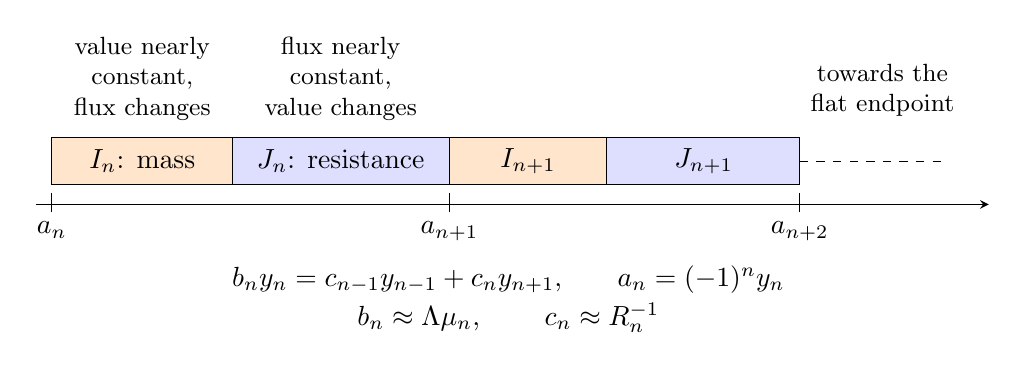
\begin{tikzpicture}[x=1cm,y=1cm,>=stealth]
\draw[->] (0,0)--(12.1,0);
\node[align=center,font=\small] at (10.75,1.45)
 {towards the\\flat endpoint};
\draw[fill=orange!20] (.2,.25) rectangle (2.5,.85);
\draw[fill=blue!13] (2.5,.25) rectangle (5.25,.85);
\draw[fill=orange!20] (5.25,.25) rectangle (7.25,.85);
\draw[fill=blue!13] (7.25,.25) rectangle (9.7,.85);
\draw[dashed] (9.7,.55)--(11.5,.55);
\node at (1.35,.55) {$I_n$: mass};
\node at (3.87,.55) {$J_n$: resistance};
\node at (6.25,.55) {$I_{n+1}$};
\node at (8.48,.55) {$J_{n+1}$};
\foreach \x/\lab in {.2/a_n,5.25/a_{n+1},9.7/a_{n+2}}
 {\draw (\x,-.1)--(\x,.15);\node[below] at (\x,-.1) {$\lab$};}
\node[align=center,font=\small] at (1.35,1.6) {value nearly\\constant,\\flux changes};
\node[align=center,font=\small] at (3.87,1.6) {flux nearly\\constant,\\value changes};
\node[align=center] at (6,-1.2)
 {$b_n y_n=c_{n-1}y_{n-1}+c_ny_{n+1}$,\qquad $a_n=(-1)^ny_n$\\[2pt]
 $b_n\approx\Lambda\mu_n$, \qquad $c_n\approx R_n^{-1}$};
\end{tikzpicture}
\caption{The intervals of a tail and the node equation satisfied by
the values $a_n$ of a solution at the entrances of the mass intervals.
Large products $\Lambda\mu_nR_n$ make successive node values of the
decaying solution small.}
\label{fig:mass-resistance-chain}
\end{figure}

\begin{lemma}[Masses and resistances of the tail]\label{lem:mass-res}
For the density $\mathsf p=wr^7$ on the tail constructed above,
\begin{equation}\label{eq:rad-eq-rm10}
 \mu_n\asymp\lambda_nA_n^2,\qquad
 R_n^I\le\frac{C}{\lambda_n}\log\frac{A_n}{B_n},\qquad
 \nu_n\le C\lambda_nA_n^6,\qquad
 R_n\asymp\frac1{\lambda_nA_n^{4}},
\end{equation}
hence
\begin{equation}\label{eq:rad-eq-rm11}
 \mu_nR_n\asymp A_n^{-2},\qquad
 \mu_nR_n^I\le CA_n^2\log\frac{A_n}{B_n},\qquad
 \nu_nR_n\le CA_n^2,
\end{equation}
and
\begin{equation}\label{eq:rad-eq-rm12}
 \log(\mu_{n+1}R_n)=2n^2+O(n^{3/2}+n).
\end{equation}
\end{lemma}

\begin{proof}
Since $dy=dr/r$ and $dr=r_X\,dX$, the measures in
\eqref{eq:mass-resistance-def-new} are $wr^6\,dr$ and $dr/(wr^8)$,
and on a model $w\,dr=\lambda r_X^2\,dX$ and $dr/w=dX/\lambda$. The
radius is bounded above and below, so \eqref{eq:rad-eq-rm6} gives
\eqref{eq:rad-eq-rm10} for the model parts. A join of length $\ell$
adds at most $W_R\ell$ to the mass and $\ell/W_L$ to the resistance of
$J_n$; relative to $\nu_n$ and $R_n$ these are
$e^{-7n^2+O(n^{3/2}+n)}$ and $e^{-11n^2+O(n)}$. The products
\eqref{eq:rad-eq-rm11} follow, and so does \eqref{eq:rad-eq-rm12}
from $\log(\lambda_{n+1}/\lambda_n)=O(n^{3/2})$ and
$\log(A_{n+1}^2/A_n^4)=2n^2+O(n)$.
\end{proof}

\paragraph{Other frequencies.}
For a general frequency the density is $\mathsf p_j$. After division
by the constant $r_\partial^{2(j^2-4)}$, where $r_\partial$ is the
radius of the endpoint,
\[
 \frac{\mathsf p_j}{\mathsf p}
 =\Bigl(\frac r{r_\partial}\Bigr)^{2(j^2-4)},
\]
and on the part of the tail beyond cell $N'$ the logarithm of this
ratio is bounded by $Cj^2A_{N'}$. So
Lemma~\ref{lem:mass-res} holds for $\mathsf p_j$, with uniform
constants, on every part of the tail where $j^2A_{N'}$ is bounded. We
shall use the slightly stronger condition
\begin{equation}\label{eq:deep-frequency-condition-new}
 j^2A_{N'}\sqrt{\log(A_{N'}/B_{N'})}\le c
\end{equation}
for a small constant $c$; by \eqref{eq:rad-eq-rm11} it makes
$\Lambda\mu_nR_n^I$ and $\Lambda\nu_nR_n$ small for all $n\ge N'$.

\subsection{The exact reduction to a recurrence}
\label{subsec:exact-reduction}

Use the coordinate $x=\log r$ at the right endpoint and $x=-\log r$ at
the left endpoint, so that $x$ always increases outward. At the left
endpoint the outward order of the intervals is
$J_N,I_N,J_{N+1},I_{N+1},\ldots$. Within this subsection only, the
resistance interval that follows $I_n$ in the outward direction is
therefore renamed $J_n$ also at the left endpoint (it is the original
$J_{n+1}$), and the first interval $J_N$ is treated as a separate
\emph{initial resistance edge} $J_0$ with resistance $R_0$ and mass
$\nu_0$. The shift of index affects only the lower-order terms of
\eqref{eq:rad-eq-rm12}.

The following definition isolates what the reduction needs.

\begin{definition}[Deep tail]\label{def:deep-tail}
Let $\mathsf p>0$ be a density on a half-line in $x$ which is divided
into consecutive intervals $I_n,J_n$ ($n\ge N'$), possibly preceded by
an initial resistance edge $J_0$, and let $\Lambda>0$. With the masses
and resistances \eqref{eq:mass-resistance-def-new} formed with $dx$,
the data form a \emph{deep tail} with constants $\eta\ll1\ll K$ if for
all $n$
\begin{equation}\label{eq:rad-eq-dg1}
 \begin{gathered}
 \Lambda\mu_nR_n^I+\Lambda\nu_nR_n\le\eta,\qquad
 \Lambda\mu_nR_n\ge K,\quad \Lambda\mu_{n+1}R_n\ge K,\\
 \nu_n\le\eta\,\min(\mu_n,\mu_{n+1}),
 \end{gathered}
\end{equation}
and if, when there is an initial edge,
$\Lambda\mu_{N'}R_0\ge K$, $\Lambda\nu_0R_0\le\eta$ and
$\nu_0\le\eta\mu_{N'}$.
\end{definition}

By Lemma~\ref{lem:mass-res} and the remark on other frequencies, the
part of a constructed tail beyond cell $N'$ is a deep tail for
$\mathsf p_j$ and $\Lambda=j^2(j^2-1)$ whenever
\eqref{eq:deep-frequency-condition-new} holds and $N'$ is large
enough; $\eta$ and $K^{-1}$ can be made as small as we wish.

\begin{lemma}[Deep inverse and the natural line]
\label{lem:radial-deep-inverse}
\label{lem:radial-flat-line}
On a deep tail, with $\eta$ and $K^{-1}$ sufficiently small, let
\[
 A_{\mathsf p}=-\mathsf p^{-1}\partial_x\,\mathsf p\,\partial_x
\]
act in $L^2(\mathsf p\,dx)$ with the Dirichlet condition at the
entrance and the Friedrichs condition at the outer endpoint.
\begin{enumerate}
\item $\|(A_{\mathsf p}-\Lambda)^{-1}\|\le C/\Lambda$.
\item Up to multiples, the equation $(A_{\mathsf p}-\Lambda)V=0$ has
 exactly one solution which is square integrable for
 $\mathsf p\,dx$ near the outer endpoint. Its values $a_n$ at the
 entrances of the mass intervals $I_n$ are nonzero and alternate in
 sign: $a_n=(-1)^ny_n$ with $y_n>0$ and
 \begin{equation}\label{eq:rad-eq-dg4}
  \frac{y_{n+1}}{y_n}
  =\frac{1+O(\eta)+O(K^{-1})}{\Lambda\mu_{n+1}R_n},
  \qquad
  \frac{\sqrt{\mu_{n+1}}\,y_{n+1}}{\sqrt{\mu_n}\,y_n}\le\frac CK<\frac12 .
 \end{equation}
\item For the constructed tails and $\mathsf p=\mathsf p_j$, the
 corresponding solution $u=r^{j^2}V$ of $L_ju=0$ is smooth and flat at
 the endpoint.
\end{enumerate}
\end{lemma}

The line spanned by the solution in (ii) is the \emph{natural line} of
Section~\ref{subsec:layout}.

\begin{proof}
The reduction is carried out on the differential equation itself, so
that the operator norm and the endpoint condition come out of one
argument. An \emph{edge} is $\mathsf E_n=I_n\cup J_n$; its two
endpoints are \emph{nodes}, and node $n$ is the entrance of $I_n$.

\step{1: one edge in the resistance coordinate}
On $\mathsf E_n$ introduce $ds=dx/\mathsf p$. The edge has length
$L_n=R_n^I+R_n$ in $s$; with $\omega=\mathsf p^2$ we have
$\mathsf p\,dx=\omega\,ds$ and
\[
 (A_{\mathsf p}-\Lambda)u=f
 \quad\Longleftrightarrow\quad -u_{ss}-\Lambda\,\omega\,u=\omega f .
\]
The Dirichlet Green function of $-\partial_s^2$ on the edge is
$G_0(s,t)=\min(s,t)\,[L_n-\max(s,t)]/L_n$. The small quantities are
\[
 \delta_n^{\rm edge}=\Lambda\int\omega(s)\,G_0(s,s)\,ds\le3\eta,
 \qquad \frac{R_n^I}{L_n}\le\frac\eta K ,
\]
by the first line of \eqref{eq:rad-eq-dg1}. The inequality
$G_0(s,z)G_0(z,t)\le G_0(s,t)G_0(z,z)$ bounds the Neumann series of
the Dirichlet Green function $G_\Lambda$ of $-\partial_s^2-\Lambda\omega$
term by term. With $l_0=1-s/L_n$, $l_1=s/L_n$, and $v_0,v_1$ the
solutions of the homogeneous equation on the edge with boundary values
$(1,0)$ and $(0,1)$, the same argument applies with one factor
replaced by $l_i$, and we obtain
\begin{equation}\label{eq:rad-eq-dg2}
 G_0\le G_\Lambda\le(1-\delta_n^{\rm edge})^{-1}G_0,
 \qquad l_i\le v_i\le(1-\delta_n^{\rm edge})^{-1}\,l_i .
\end{equation}
For $u$ vanishing at both ends of the edge,
$\Lambda\int\omega|u|^2\le\delta_n^{\rm edge}\int|u_s|^2$. Hence the
direct sum $G_D$ of the Dirichlet inverses of all edges has norm at
most $C\eta/\Lambda$ on $L^2(\mathsf p\,dx)$.

\step{2: the boundary matrix of an edge}
For boundary values $(a,a')$ at the two ends of $\mathsf E_n$ the
homogeneous solution is $av_0+a'v_1$, and its outward derivatives at
the two ends, in the variable $s$, are given by the matrix
\[
 \begin{pmatrix}d_{n,0}&-c_n\\-c_n&d_{n,1}\end{pmatrix},\qquad
 c_n=\frac1{L_n}+\Lambda\int\omega\,l_0v_1,\qquad
 d_{n,i}=\frac1{L_n}-\Lambda\int\omega\,l_iv_i ;
\]
the formulas follow from Green's identity with the functions $l_i$.
Since $l_0l_1=G_0(s,s)/L_n$, \eqref{eq:rad-eq-dg2} gives
\begin{equation}\label{eq:rad-eq-dg3}
 c_n=\frac{1+O(\eta)}{R_n},\qquad
 b_n:=-d_{n-1,1}-d_{n,0}
       =\Lambda\mu_n\,\bigl(1+O(\eta)+O(K^{-1})\bigr).
\end{equation}
For the second formula: on $I_n$ we have $l_0=1+O(R_n^I/L_n)$, so
that interval contributes $\Lambda\mu_n(1+O(\eta))$ to
$\Lambda\int\omega\,l_0v_0$, and $J_n$ contributes at most
$C\Lambda\nu_n\le C\eta\Lambda\mu_n$. The preceding edge contributes
to $\Lambda\int\omega\,l_1v_1$ at most $C\Lambda$ times
$\nu_{n-1}+\mu_{n-1}(R_{n-1}^I/L_{n-1})^2$, and the second term is at
most $\eta^2K^{-2}\mu_n$ by \eqref{eq:rad-eq-dg1}. The two terms
$1/L_n$ and $1/L_{n-1}$ are at most $\Lambda\mu_n/K$ each. The same
computation covers an initial resistance edge.

\step{3: interpolation of node values}
For a sequence $a=(a_n)$ of node values let $Ta$ be the function which
on each edge is the homogeneous solution with these boundary values,
$(Ta)|_{\mathsf E_n}=a_nv_0+a_{n+1}v_1$. Let
$\mathfrak h=\ell^2(\mu_n)$. Then
\begin{equation}\label{eq:rad-eq-dj1}
 c\,\|a\|_{\mathfrak h}^2\le\|Ta\|_{L^2(\mathsf p\,dx)}^2
                         \le C\,\|a\|_{\mathfrak h}^2 .
\end{equation}
Indeed, by \eqref{eq:rad-eq-dg2} the function $Ta$ is close to $a_n$
on $I_n$, which carries the mass $\mu_n$. On $I_n$ the neighbouring
value enters with the factor $l_1\le R_n^I/L_n$, and the sum of these
contributions is $O(\eta^2/K^2)\,\|a\|_{\mathfrak h}^2$ after a shift
of index. The contribution of $J_n$ is controlled by the last
inequality of \eqref{eq:rad-eq-dg1}.

\step{4: the node operator}
The quadratic form of $A_{\mathsf p}-\Lambda$ on interpolants is, by
Step~2,
\[
 (\mathcal Da,a)_{\mathfrak h}
   =-\sum_n b_n|a_n|^2-2\operatorname{Re}\sum_n c_n\,a_n\overline{a_{n+1}} ,
\]
which defines a symmetric operator $\mathcal D$ on $\mathfrak h$. In
the coordinates $\sqrt{\mu_n}\,a_n$ its diagonal entries have size
$\Lambda$ by \eqref{eq:rad-eq-dg3}, while each off-diagonal entry is
bounded by $C/(R_n\sqrt{\mu_n\mu_{n+1}})\le C\Lambda/K$. By diagonal
dominance
\[
 \|\mathcal D^{-1}\|\le\frac C\Lambda ,
\]
independently of the number of edges.

\step{5: the inverse}
These algebraic facts give an inverse of the operator because they
respect its form domain. On the one hand, the energy of an interpolant
is bounded by $C\Lambda\|a\|_{\mathfrak h}^2$, by the formula for
$\mathcal D$ and \eqref{eq:rad-eq-dj1}. On the other hand, averaging
$u(x_n)-u(x)$ over $I_n$, where $x_n$ is node $n$, gives
\[
 \mu_n\,|u(x_n)|^2\le2\,\|u\|_{L^2(I_n,\mathsf p\,dx)}^2
            +2\mu_nR_n^I\int_{I_n}|u_s|^2\,ds ,
\]
so every function in the form domain has node values in $\mathfrak h$
and splits as $u=Ta+u^\circ$ with $u^\circ$ vanishing at all nodes.
The two parts are orthogonal for the form of $A_{\mathsf p}-\Lambda$,
because $Ta$ solves the homogeneous equation on each edge. Therefore
\begin{equation}\label{eq:rad-eq-dj2}
 (A_{\mathsf p}-\Lambda)^{-1}=G_D+T\,\mathcal D^{-1}T^*,
 \qquad (T^*f)_n=\frac1{\mu_n}\int\mathsf p\,(T\mathbf e_n)\,f\,dx ,
\end{equation}
where $\mathbf e_n$ is the $n$th unit sequence. Truncations of the
tail by a Dirichlet wall at a far node obey the same formula and
converge strongly, since the diagonally dominant series for
$\mathcal D^{-1}$ converges uniformly on finite compressions; their
limit is the Friedrichs realization identified by the decomposition
of the form domain. Steps~1, 3 and~4 now give~(i).

\step{6: the decaying solution}
A homogeneous solution is the interpolant of its node values, and
continuity of the flux at node $n$ reads
$-b_na_n=c_{n-1}a_{n-1}+c_na_{n+1}$. With $a_n=(-1)^ny_n$ this is
\[
 b_n\,y_n=c_{n-1}\,y_{n-1}+c_n\,y_{n+1}.
\]
Put $\epsilon_n=c_n^2/(b_nb_{n+1})\le C/K^2$ and
$t_n=b_{n+1}y_{n+1}/(c_ny_n)$. Eliminating backwards from the outer
end,
\[
 t_n=\frac1{1-\epsilon_{n+1}t_{n+1}} .
\]
For large $K$ these maps preserve the interval $[1,2]$ and contract
it by a factor at most $\tfrac12$. Hence the solutions with a
Dirichlet wall at a far node converge, as the wall recedes, to a
unique sequence with $t_n\in[1,2]$ for all $n$. By
\eqref{eq:rad-eq-dg3} it satisfies \eqref{eq:rad-eq-dg4}, and by
\eqref{eq:rad-eq-dj1} its interpolant is square integrable.

Any solution independent of this one has node values of the form
\[
 z_n=y_n\Bigl(C+\mathcal W\sum_{k<n}\frac1{c_ky_ky_{k+1}}\Bigr),
 \qquad\mathcal W\ne0 .
\]
Consecutive terms of the sum grow by a factor at least $cK^2$, so
eventually $|z_{n+1}/z_n|\asymp\Lambda\mu_nR_n$ and
$\sqrt{\mu_{n+1}}\,|z_{n+1}|\ge cK\sqrt{\mu_n}\,|z_n|$. On $I_n$ the
contribution of the neighbouring node is at most $C\eta$ times that of
node $n$ itself, so the $L^2(\mathsf p\,dx)$ norm of this solution
diverges. This proves the uniqueness in~(ii); in the language of
Sturm--Liouville theory, the outer endpoint is of limit-point type.

\step{7: flatness for the constructed tails}
Summing \eqref{eq:rad-eq-rm12} in \eqref{eq:rad-eq-dg4} gives, for
$k\ge m$,
\begin{equation}\label{eq:rad-eq-rm17}
 \left|\frac{a_k}{a_m}\right|
 \le\mathcal E_k^C\,\mathcal E_m^C\,e^{-(S_k-S_m)},
 \qquad\text{since}\quad
 2\sum_{n=m}^{k-1}n^2
 =\tfrac23(k^3-m^3)-(k^2-m^2)+\tfrac13(k-m),
\end{equation}
where the accumulated errors $O(n^{3/2}+n)$ and the quadratic terms
are absorbed by $q_k+q_m$. By Lemma~\ref{lem:tail-flat} every radial
derivative of fixed order costs at most $e^{C_sn^2}$ on cell $n$, and
the normalized gauge factor $(r/r_\partial)^{j^2}$ is bounded with
bounded inverse in the range \eqref{eq:deep-frequency-condition-new}.
Thus, after a normalization at the entrance, the solution and all its
derivatives of fixed order are bounded on cell $n$ by
$\mathcal E_n^{C_s}e^{-S_n}$, which tends to zero faster than every
power of $d_\partial$. This is~(iii).
\end{proof}

\begin{remark}\label{rem:line-continuity}
The contraction in Step~6 is uniform in the height ratios, so the
natural line depends continuously on $(\sigma_k)_{k\ge N}$ in the
product topology. This is used in
Lemma~\ref{lem:radial-product-selection}.
\end{remark}

\subsection{Localized bounds for the deep inverse}
\label{subsec:deep-green}

Later we need more than the operator norm: the kernel of the deep
inverse decays between distant cells.

\paragraph{The node Green matrix.}
Let $\mathsf N$ be the symmetric tridiagonal matrix with diagonal
entries $b_n$ and off-diagonal entries $-c_n$. Up to the signs
$(-1)^n$ and the weights $\mu_n$ it represents $-\mathcal D$, and by
Step~4 it is positive with a bounded inverse in the coordinates
$\sqrt{\mu_n}\,a_n$. Let $\Gamma=\mathsf N^{-1}$. Its diagonal
satisfies $b_m^{-1}\le\Gamma_{mm}\le Cb_m^{-1}$, by the Neumann series
with positive terms. For fixed $m$ the sequence $n\mapsto\Gamma_{nm}$,
$n\ge m$, is a decaying solution of the recurrence, so by uniqueness
\begin{equation}\label{eq:rad-eq-dj4}
 \Gamma_{nm}=\Gamma_{mm}\,\frac{y_n}{y_m}
 \le\frac{C}{\Lambda\mu_m}
      \prod_{k=m}^{n-1}\frac{1+C(\eta+K^{-1})}{\Lambda\mu_{k+1}R_k}
 \qquad(n\ge m),
\end{equation}
and symmetry gives the bound for $n<m$. The kernel of
$T\mathcal D^{-1}T^*$ in \eqref{eq:rad-eq-dj2} is built from $\Gamma$
with additional signs, which do not matter for absolute bounds, and
with at most two interpolation functions at each of its two
arguments; the kernel of $G_D$ lives on single edges. With
\eqref{eq:rad-eq-rm17} we conclude: for the constructed tails, the
part of the kernel of $(A_{\mathsf p}-\Lambda)^{-1}$ leading from cell
$m$ to cell $n$ has operator norm at most
\begin{equation}\label{eq:rad-eq-dj5}
 C\,\mathcal E_n^C\,\mathcal E_m^C\,e^{-|S_n-S_m|}.
\end{equation}

\paragraph{Return to radial units.}
Let $g=(r/r_\partial)^{j^2}$ and $\mathsf p^\circ=g^2w/r$, a constant
multiple of $\mathsf p_j$. By Lemma~\ref{lem:gauge},
\[
 L_j(gV)=-\frac{gw}{r^2}\,(A_{\mathsf p^\circ}-\Lambda)V,
 \qquad \mathsf p^\circ\,dx=\frac{g^2w}{r^2}\,dr,
 \qquad G_{L_j}(r,r')=-g(r)\,g(r')\,G_A(x,x'),
\]
where $G_{L_j}$ and $G_A$ are the kernels of the inverses of $L_j$,
with respect to $dr$, and of $A_{\mathsf p^\circ}-\Lambda$, with
respect to $\mathsf p^\circ dx$. The gauge factors are bounded above
and below, so \eqref{eq:rad-eq-dj5} holds for the inverse of $L_j$ in
the $dr$ pairing. In terms of the operator $B_j=-\varpi^{-1}L_j$ of
\eqref{eq:rad-eq-ha2},
\begin{equation}\label{eq:rad-eq-rm20}
 B_j=\frac1{12}\,g\,\bigl(A_{\mathsf p_j}-j^2(j^2-1)\bigr)\,g^{-1},
 \qquad \|B_{j,D}^{-1}\|\le\frac{C}{j^{4}}
\end{equation}
on a deep tail, where $B_{j,D}$ has the Dirichlet condition at the
entrance.

\paragraph{The entrance impedance.}
For the natural solution, the boundary matrix of Step~2 gives at a
mass entrance
$\mathsf pV_x/(\Lambda\mu_nV)=1+O(\eta)+O(K^{-1})$; if an initial
resistance edge comes first, the ratio of flux to value is instead
$-(1+O(\eta)+O(K^{-1}))/R_0$. In both cases the boundary term of
Green's identity at the outer endpoint vanishes for the natural
solution: at node $n$ it is bounded by $C\Lambda\mu_n|a_n|^2\to0$,
and finiteness of mass and energy identifies this with the limit at
the endpoint.

\subsection{Frequency bands: one transition cell at every frequency}
\label{subsec:bands}

How a cell acts on a solution depends on the frequency. If the action
$\tau_{n,j}=j\sqrt{A_n}$ of its caps is large, the cell is isolated
from its neighbours and is governed by its own spectral gap
(Lemma~\ref{lem:morse-arithmetic}). If the condition
\eqref{eq:deep-frequency-condition-new} holds, the cell is part of a
deep tail and is governed by the recurrence. The following
definition arranges that, at each frequency, at most one cell at each
end falls between the two regimes. Fix a large constant $C_*$ and put
\begin{equation}\label{eq:rad-eq-rm21}
 \jn_n=C_*\,q_n\,A_n^{-1/2},\qquad
 \mathcal I_n=\{j\ \text{even}:\ \jn_{n-1}\le j<\jn_n\}\quad(n>N),
\end{equation}
and let the first band $\mathcal I_N$ consist of all even $j$ with
$2\le j<\jn_N$. The \emph{bands} $\mathcal I_n$, $n\ge N$, partition
the even frequencies. For $j\in\mathcal I_n$:
\begin{itemize}
\item every earlier cell $m<n$ has large action,
 $\tau_{m,j}=j\sqrt{A_m}\ge C_*q_m$. These cells, together with the
 central model, form the \emph{inner region};
\item cell $n$ is the \emph{transition cell};
\item the cells $m>n$ form a deep tail, because
 \begin{equation}\label{eq:rad-eq-rm22}
  j^2A_{n+1}\sqrt{\log(A_{n+1}/B_{n+1})}
  \le C\,C_*^2\,q_n^2\,\frac{A_{n+1}}{A_n}\,(n+1)\longrightarrow0 .
 \end{equation}
\end{itemize}
So there is no range of frequencies left unexamined between the local
spectral inverses and the deep inverse. The decomposition depends on
the frequency; the profile does not. This structure is the key to the
assembly of the global inverse in
Section~\ref{sec:radial-reference-inverse}.

\paragraph{An auxiliary cone at the entrance of a tail.}
To define an incoming line for the first band, attach at the entrance
of each tail an auxiliary cone $w=cr$. For the right tail the cone is
continued inward to $r=0$, for the left tail outward to $r=\infty$.
The transition between cone and first cell is a short positive
interval with $rw'/w\ge1$, constructed by applying
\eqref{eq:rad-eq-rm8} to $\log(w/r)$. On the cone, in $y=\log r$,
\[
 B_j=\tfrac1{12}\,(-\partial_y^2+j^2),\qquad
 \varpi\,dr=12c\,dy ;
\]
the solutions regular at the far end of the cone are $r^{j}$ for the
right tail and $r^{-j}$ for the left tail, and the Dirichlet inverse
of $B_j$ has norm at most $12/j^2$. The cone serves only to specify
an incoming line. The final profile retains a finite piece of it, the
\emph{cone head}.

\subsection{Choosing the heights so that the lines do not meet}
\label{subsec:height-selection}

Fix an endpoint, a band index $n$ and a frequency
$j\in\mathcal I_n$. Consider the join which precedes cell $n$ in the
outward order (for $n=N$: the transition from the auxiliary cone).
Let $W_{\rm in}$ be the value of the profile at its inner end and
$\sigma_nW^0_{\rm out}$ its value at the outer end. By
\eqref{eq:rad-eq-js2}, $W_{\rm in}$ does not depend on $\sigma_n$,
and $W^0_{\rm out}$ is the outer value for $\sigma_n=1$. Put
\begin{equation}\label{eq:rad-eq-js4}
 \Xi_n=\frac{W^0_{\rm out}}{W_{\rm in}},\qquad
 \Upsilon_n=\max(\Xi_n,\Xi_n^{-1}),\qquad
 \log\Upsilon_n=4n^2+O(n^{3/2}+n).
\end{equation}
At the first join the amplitude $c$ of the auxiliary cone is chosen,
independently of $\sigma_N$, so that the contrast is the same. The
radii and all cut points are independent of the height ratios.

The role of $\sigma_n$ is the following. Everything beyond the join is
multiplied by $\sigma_n$; this does not change the homogeneous
equation there, hence not the natural line. The incoming line is
determined by what lies before the join, and does not depend on
$\sigma_n$ either. What $\sigma_n$ changes is the scale of the flux
$wu'$ by which the two lines are compared across the join. We show
that this is enough to move them apart.

\paragraph{A state variable adapted to the join.}
On a join $w'/w$ is huge, and the pair $(u,wu')$ is not a convenient
state. Define instead
\begin{equation}\label{eq:rad-eq-js5}
 \zeta_j=\frac{ru_r}{j^2}-u .
\end{equation}
If $L_ju=0$, then $(w\zeta_j)'=-(j^2-1)\,wu_r/j^2$, in which $w'$ no
longer appears. For the state
$Y=(u,\ w\zeta_j/W_{\rm in})$ this gives
\begin{equation}\label{eq:rad-eq-js7}
 Y_r=\frac1r
 \begin{pmatrix}
 j^2&j^2\,W_{\rm in}/w\\
 -(j^2-1)\,w/W_{\rm in}&-(j^2-1)
 \end{pmatrix}Y .
\end{equation}
The coefficients involve only the sizes of $w$ and $w^{-1}$ on the
join, which lie between those at its ends. By the Volterra series,
the transfer matrix of \eqref{eq:rad-eq-js7} across the join differs
from the identity by at most $e^{\eta_{n,j}}-1$, where
\begin{equation}\label{eq:rad-eq-js14}
 \eta_{n,j}=Cj^2\,\frac{\ell_n}{r_{\min}}\,\Upsilon_n
 \le C\,C_*^2\,q_n^2\,e^{-7n^2+O(n^{3/2}+n)}=o(e^{-n^2}),
\end{equation}
$\ell_n$ being the length of the join. This is the computation behind
the exponent $12$ in \eqref{eq:rad-eq-rm7}: the steepness of the
profile on the join causes no difficulty.

\paragraph{The incoming line has a definite slope.}
As a stand-in for the incoming line we use the solution which vanishes
at a cut inside the positive cap preceding the join. The true incoming
line differs from it by an exponentially small amount, which is
accounted for in Section~\ref{subsec:terminal-matching}. Normalize
this solution to $u=1$ at the join. Then
\begin{equation}\label{eq:rad-eq-js6}
 a:=\frac{\zeta_j}{u}\in\bigl[-\tfrac32,-\tfrac12\bigr].
\end{equation}
Indeed, on the cap $u_{XX}=j^2|\rho|\,u$, and comparison with the
Riccati equation for a constant potential gives
$|u_X/u|\le Cj\sqrt b\,\coth(cj\sqrt A)$, where $b$ is the size of
$|\rho|$ on the cap and $A=A_{n-1}$. The cap is either the short one,
with $|\rho|\asymp A$, length $\asymp1$ in $X$ and $r_X\asymp A$, or
the long one, with $|\rho|\asymp A^9$, length $\asymp A^{-4}$ and
$r_X\asymp A^5$. In both cases $r_X\asymp\sqrt{Ab}$, so
\[
 \Bigl|\frac{ru_r}{j^2u}\Bigr|\le\frac{C}{j\sqrt{A_{n-1}}}<\frac12
\]
once $C_*$ is large, because $j\sqrt{A_{n-1}}\ge C_*q_{n-1}$. At the
left endpoint only the sign of $ru_r$ changes. In the first band the
cone gives $ru_r/(j^2u)=\pm1/j$, which is at most $\tfrac12$ in
absolute value even for $j=2$.

\paragraph{The excluded set of height ratios.}
Let $(\beta_1,\beta_2)$ span the natural line in the frame
$(u,\zeta_j)$ at the outer end of the join, computed for
$\sigma_n=1$. In the common frame $Y$ the natural line is then spanned
by
\[
 \mathbf b(\sigma)=(\beta_1,\ \sigma\,\Xi_n\,\beta_2),
 \qquad \sigma=\sigma_n ,
\]
while the stand-in for the incoming line is spanned by $(1,a)$; see
Figure~\ref{fig:height-selection}. If $\beta_1=0$ the angle between
the two lines is bounded below. Otherwise put
$b_\sigma=\sigma\Xi_n\beta_2/\beta_1$; the sine of the angle is
\[
 \frac{|a-b_\sigma|}{\sqrt{1+a^2}\,\sqrt{1+b_\sigma^2}} .
\]
If this is small, $b_\sigma$ lies in a fixed compact interval of
negative numbers, on which $|db_\sigma/d\sigma|=|b_\sigma|/\sigma$ is
bounded below. Therefore the set of $\sigma\in[1,2]$ for which the
sine is less than $2\delta_n$, with
\[
 \delta_n=c_0\,e^{-n^2},
\]
is contained in an interval of length at most $C\delta_n$. The state
of the stand-in solution after crossing the join is
$(1,a)+O(\eta_{n,j})$, and normalization of vectors is Lipschitz near
$(1,a)$. By \eqref{eq:rad-eq-js14} the same conclusion holds for the
angle after the join: \emph{the set of $\sigma_n\in[1,2]$ for which
the incoming and natural lines make an angle of sine less than
$\delta_n$ lies in an interval of length at most $C\delta_n$.} The
constant does not depend on $j$ or on the other height ratios,
however large or small the contrast $\Xi_n$ may be.

\begin{figure}[htbp]
\centering
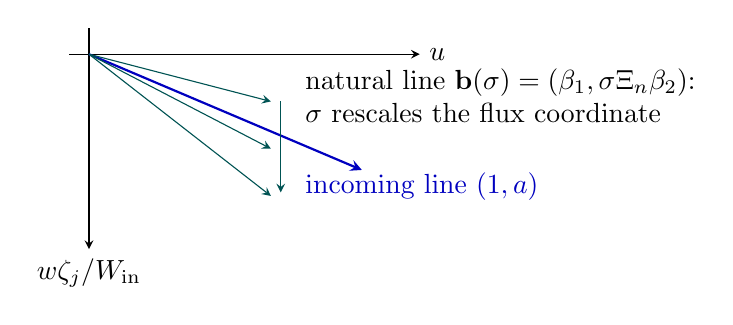
\begin{tikzpicture}[x=2.1cm,y=1.5cm,>=stealth]
\draw[->] (-.12,0)--(2,0) node[right] {$u$};
\draw[->] (0,.22)--(0,-1.65) node[below] {$w\zeta_j/W_{\rm in}$};
\draw[thick,blue!75!black,->] (0,0)--(1.65,-.98);
\node[anchor=west,blue!75!black] at (1.25,-1.12) {incoming line $(1,a)$};
\draw[teal!65!black,->] (0,0)--(1.1,-.4);
\draw[teal!65!black,->] (0,0)--(1.1,-.8);
\draw[teal!65!black,->] (0,0)--(1.1,-1.2);
\draw[->,teal!65!black] (1.16,-.4)--(1.16,-1.17);
\node[anchor=west,align=left] at (1.25,-.35)
 {natural line $\mathbf b(\sigma)=(\beta_1,\sigma\Xi_n\beta_2)$:\\
  $\sigma$ rescales the flux coordinate};
\end{tikzpicture}
\caption{Selection of a height ratio in the plane of boundary states.
The slope of the incoming line lies in a fixed negative interval.
As $\sigma$ varies, the natural line sweeps past it with speed bounded
below, so the two lines are close only for a short interval of
$\sigma$.}
\label{fig:height-selection}
\end{figure}

\begin{lemma}[Simultaneous selection of the heights]
\label{lem:radial-product-selection}
If $N$ is large enough, then at each endpoint the height ratios
$\sigma_n\in[1,2]$, $n\ge N$, can be chosen so that for every $n$ and
every $j\in\mathcal I_n$ the incoming and natural lines at the join
preceding cell $n$ make an angle of sine at least
$\delta_n=c_0e^{-n^2}$ in the state \eqref{eq:rad-eq-js7}.
\end{lemma}

\begin{proof}
The band $\mathcal I_n$ contains at most
$\jn_n=C_*q_ne^{n^2/2}(1+o(1))$ frequencies, so the total length of
the excluded intervals satisfies
\begin{equation}\label{eq:rad-eq-js13}
 \sum_{n\ge N}C\,\#\mathcal I_n\,\delta_n
 \le C\,C_*c_0\sum_{n\ge N}q_n\,e^{-n^2/2}<\frac12
\end{equation}
for large $N$. The excluded interval for a pair $(n,j)$ depends on
the ratios $\sigma_k$ with $k\ne n$, but the bound for its length does
not, and this is all we need.

Consider first finitely many bands $N\le n\le N_1$, with
$\sigma_k=1$ for $k>N_1$, and Lebesgue measure on the cube
$[1,2]^{N_1-N+1}$. By Fubini's theorem and the uniform
one-dimensional bound, the set of ratios violating the condition for a
given pair $(n,j)$ has measure at most $C\delta_n$, and by
\eqref{eq:rad-eq-js13} the union of these sets has measure less than
one. So a good choice exists for every $N_1$. Extend each of these
choices by ones and pass to a subsequence converging in every
coordinate. For a fixed frequency, the transfer across finitely many
cells is continuous in the ratios, and the natural line is continuous
in the product topology by Remark~\ref{rem:line-continuity}. Each
condition on the angle is closed, hence holds for the limit. The two
endpoints are treated independently.
\end{proof}

\subsection{Summary}

We have constructed, at each endpoint, a smooth flat tail with the
following properties, for every even frequency $j$ with band index
$n$: beyond cell $n$ the equation $L_ju=0$ has a unique decaying
solution, which is flat at the endpoint, and $L_j$ has a Dirichlet
inverse with the localized bound \eqref{eq:rad-eq-dj5}; at the
entrance of cell $n$ the natural line makes an angle at least
$\delta_n$ with the line arriving through the preceding positive cap.

We have \emph{not} yet shown that gluing the tails to the central
model preserves the spectral gaps of the pieces. That global question
is the subject of the next section. Its answer uses both halves of the
present construction: the selected angle at the transition cell, and
the strong attenuation through the positive cap that precedes it.
